\begin{comment}
\addbibresource{referencias/Referencias.bib}
\end{comment}

\section{Metodología}
\label{sc:metodos}
	En orden de cumplir con los objetivos propuestos en el capítulo \ref{sc:objetivos}, se plantea una implementación de NL-FEM. Para ello, se parte de la metodología propuesta en \textit{\citetitle*{Pisano2009}} \parencite{Pisano2009} que sigue la ecuación constitutiva planteada en el capítulo \ref{sc:teoria}
	\subsection{Implementación Elasticidad No Local}
	\label{sub:implementación}
	Para llegar a la implementación se parte de la implementación clásica (local) de FEM. Para efectos de este estudio se asumen esfuerzos planos, por lo que:
	\begin{subequations}
		\begin{equation}
			\sigma_{xz}=0
		\end{equation}
		\begin{equation}
			\sigma_{yz}=0
		\end{equation}
		\begin{equation}
			\sigma_{z}=0
		\end{equation}
	\end{subequations}
	Lo cual permite expresar el tensor de rigidez $C$ como:

	\begin{equation}
	\boldsymbol{C}=
		\begin{pmatrix}
			C_{11} & C_{12} & 0\\
			C_{12} & C_{11} & 0\\
			0 & 0 & C_{66}\\
		\end{pmatrix}
	\end{equation}

	Donde:

	\begin{subequations}
		\begin{equation}
			C_{11}=\frac{E}{1-v^2}
		\end{equation}
		\begin{equation}
			C_{12}=\frac{vE}{1-v^2}
		\end{equation}
		\begin{equation}
			C_{66}=\frac{E}{2(1+v)}
		\end{equation}
	\end{subequations}

		\subsubsection{Método FEM}
		Se parte de la metodología planteada en \textcite{Reddy} donde se divide el método en 6 pasos:
			\begin{enumerate}
				\item Enmallado:

				Se divide el dominio en elementos y se enumeran sus nodos con grados de libertad. Para el caso de elasticidad, se deben tener dos grados de libertad por nodo. El primero pertenece al desplazamiento en x,comunmente llamado $U$ y el segundo pertenece al desplazamiento en y, comunmente llamado $V$. El número de nodos por elemento depende del orden de aproximación y de la geometría del elemento. Para este estudio se usarán elementos de cuatro lados con 8 nodos por elemento, comúnmente llamados \textit{Serendipity Elements} y elementos triangulares con 6 nodos.
				\item Ecuaciones a nivel de elemento

				Mediante un modelo de elementos finitos (al que se puede llegar con la forma débil de la ecuación diferencial) se realiza el proceso de integración de las matrices de coeficientes, fuerzas nodales y flujos por elemento. Generalmente la integración se realiza usando la cuadratura de Gauss-Legendre.
				\item Ensamblaje

				Se obliga a la solución a ser continua en todo el dominio y se asegura el equilibrio de flujos en los nodos. Esto genera un sistema de ecuaciones el cual se ensambla mediante las matrices y vectores encontrados en el paso anterior. 
				\item Imposición de condiciones de borde

				Se imponen condiciones de borde operando matricialmente los valores conocidos para la solución o asignando directamente el flujo conocido al sistema de ecuaciones. 
				\item Solución

				Se soluciona el sistema de ecuaciones encontrando la solución en cada grado de libertad.
				\item Post - Proceso

				Se calcula el gradiente de la solución (variables secundarias) y se reportan los resultados de manera gráfica.

			\end{enumerate}
		\subsubsection{Modificaciones No Locales}
		Para la inclusión de la no localidad se deben modificar los 3 primeros pasos del método clásico. Estos cambios se deben a la inclusión de una integral convolutiva en la ecuación constitutiva y a la elección de la función de atenuación.
			\begin{enumerate}
				\item Enmallado

				Uno de los cambios mas relevantes en el proceso de NL-FEM es la inclusión de los elementos no locales por cada elemento local. Para ello, la literatura se propone encontrar los elementos cuyos centroides se encuentren dentro de una distancia de influencia $Lr$ \parencite{article}, sin embargo, \textcite{ProgramaEnmallado} sugiere que el proceso de selección de elementos no locales debe tener en cuenta la distancia adicional que se tenga al punto mas alejado del elemento. En la figura \ref{fig:nolocales_lr_cambios} se muestran gráficamente ambos procesos.

				\begin{figure}
					\centering
					\sffamily
					\includegraphics[width=\textwidth]{figuras/diferenciasLr.pdf}
					\caption{Cambios en la inclusión de elementos no locales. Se evalúa el elemento 63. El círculo azul representa un radio de $Lr=6*l$ con $l=0.1$ desde el centroide del elemento}
					\label{fig:nolocales_lr_cambios}
				\end{figure}

				Dadas las propiedades de las funciones de atenuación descritas en el capítulo \ref{sc:teoria}, se puede asegurar que si se toma una distancia $Lr\rightarrow\infty$ el resultado no cambia de manera significante. En caso de que no se disponga de un algoritmo que reconozca los elementos no locales, esto simplifica el proceso de enmallado. En caso de que se tenga $Lr\rightarrow\infty$ el costo computacional aumenta severamente, por lo que se aconseja siempre identificar los elementos no locales.

				Para este estudio se tomara $Lr$ variable, pero nunca menor de $6l$ como se expuso en el capítulo \ref{sc:teoria}

				En conclusión, en un dominio de$N$ elementos se conoce que: Para cada elemento $n_i$ existe un numero $M$ de elementos no locales $m_j$. $M$ varía para cada elemento pues depende de su posición en el dominio.
				\item Ecuaciones a nivel de elemento

				Como se expuso en el capítulo \ref{sc:teoria}, se debe realizar una integral convolutiva en el proceso de integración. Por lo tanto, por cada elemento se obtiene una matriz local y un numero específico de matrices no locales.

				La matriz local se obtiene usando la teoría clásica (local) de elasticidad.

				Las matrices no locales se encuentran usando el modelo propuesto por \textcite{Pisano2009} donde:
				\begin{equation}
					\boldsymbol{k_{nm}^{nloc}}=\int_{V_n}\int_{V_m}{A(|\boldsymbol{x}-\boldsymbol{x'}|/l)\boldsymbol{B_n^T}(\boldsymbol{x})\boldsymbol{D}\boldsymbol{B_n}(\boldsymbol{x})}{dV'}{dV}
					\label{eq:nl_1}
				\end{equation}
				Donde:
				\begin{enumerate}
					\item[] $n$ se refiere al elemento local.
					\item[] $m$ se refiere al elemento no local.
					\item[] $A$ es la función de atenuación.
					\item[] $\boldsymbol{B_n}$ es la matriz de derivadas parciales de las funciones de forma.
					\item[] $\boldsymbol{D}$ tensor de rigidez.
					\item[] $\boldsymbol{x}$ representa un punto del elemento local $n$.
					\item[] $\boldsymbol{x'}$ representa un punto del elemento no local $m$.
				\end{enumerate}
				En la terminología de \textcite{Reddy} se puede reescribir esta ecuación a nivel de elemento separando los desplazamientos en x y y en submatrices de la matriz del elemento. Como ejemplo se muestra la matriz $\boldsymbol{K_{uu}}$:
				\begin{equation}
					\boldsymbol{UU_{nm}^{nloc}}[i,j]=t^2\int_{\Omega_n}\int_{\Omega_m}{A(\rho)\left[C_{11}\frac{\partial \psi_i^{l}}{\partial x}\frac{\partial \psi_j^{nl}}{\partial x}+C_{66}\frac{\partial \psi_i^{l}}{\partial y}\frac{\partial \psi_j^{nl}}{\partial y}\right]}{d\Omega_m}{d\Omega_n}
				\label{eq:nl_2}
				\end{equation}
				Notese que a la ecuación \ref{eq:nl_1} es una integral volumétrica, mientras que la ecuación \ref{eq:nl_2} corresponde a una integral de área, por tal razon, se debe multiplicar por el grosor al cuadrado.

				Donde:
				\begin{enumerate}
					\item[] $\rho$ es la relación $|\boldsymbol{x}-\boldsymbol{x'}|/l$.
					\item[] $\psi_i$ es la i-ésima función de forma.
					\item[] $C_{11},C_{66}$ son los componentes del tensor elástico para esfuerzos planos.
					\item[] El super índice $^l$ significa que la función pertenece al elemento local.
					\item[] El super índice $^{nl}$ significa que la función pertenece al elemento no local.
					\item[] Las funciones estan evaluadas en los puntos correspondientes a su elemento, es decir, la función $\psi_i^{nl}$ esta evaluada en los puntos $x_{nl},y_{nl}$
				\end{enumerate}
				En los anexos \ref{eq:anexos.matrices_elementos} se encuentra el desarrollo de las otras submatrices.
				\item Ensamblaje

				Dado que los elementos no locales tienen aportaciones a la matriz general del sistema, el ensablaje de dichos elementos debe tenerse en cuenta usando los grados de libertad de los elementos correspondientes. Por ejemplo, si se evalúa la matriz no local del elemento local 3 con respecto al elemento 4, en la matriz del sistema se debe incluir este aporte el las filas que correspondan a los grados de libertad del elemento 3 con las columnas que representen los grados de libertad del elemento 4. Esta generalización hace posible que se puedan tener combinación de diferentes tipos de elementos (como elementos triangulares y rectangulares).
			\end{enumerate}
		\subsubsection{Estructura del Programa}
		La implementación computacional propuesta consta de 2 módulos, el módulo procesador y el módulo integrador. La implementación completa se encuentra en \href{https://github.com/ZibraMax/NLFEM}{GitHUB}. 
			\begin{enumerate}
				\item Módulo Procesador

				El módulo procesador esta escrito en Python y requiere de las librerías \textit{triangle}, \textit{NumPy} y \textit{Matplotilib}. Este módulo se puede encargar de la solución completa de un problema de NL-FEM.
				Para el enmallado se usa el \textit{wrapper} de \textit{triangle} \parencite{triangle}, que lleva el mismo nombre. Fue desarrollado por \href{https://rufat.be/index.html}{Dzhelil Rufat} y consta de una serie de funciones que realiza triangulaciones \textit{Delauney}. El enmallado por \textit{triangle} no suele ser uniforme, ya que en el proceso los elementos son refinados para obligar a que los ángulos de los triángulos no sean menores a 35 grados.
				Adicionalmente \textcite{ProgramaEnmallado} desarrolló un algoritmo para realizar el proceso de enmallado en dominios rectangulares identificando elementos no locales a una distancia $Lr$. Esto facilitó el proceso de enmallado para los casos de estudio propuestos.

				Para las ecuaciones a nivel de elemento se usa la ecuación \ref{eq:nl_2} y sus variaciones en el anexo \ref{eq:anexos.matrices_elementos}.

				Para la integración se usa la cuadratura de Gauss Legendre. Se puede integrar con cualquier número de puntos. Los puntos y pesos se extraen de la librería \href{https://numpy.org/doc/stable/reference/generated/numpy.polynomial.legendre.leggauss.html}{NumPy}.

				Para el ensamblaje de matrices y vectores se usan las propiedades de los arreglos de \textit{NumPy}.

				Para las condiciones de borde se crearon métodos auxiliares que permiten generar las condiciones en los nodos que pertenezcan a segmentos y nodos que se encuentren en puntos (coordenadas) específicos. Los segmentos pueden ser definidos por el usuario o ser generados automáticamente por el programa. Esto se realizó ya que las condiciones de borde generalmente se asignan en los contornos del dominio.
				
				Las condiciones de borde se toman como listas nativas de Python, lo que permite que se puedan manejar de manera sencilla. Un ejemplo es tener condiciones de borde en dos segmentos distintos. Para poder concatenarlas y que el programa reconzca y aplique ambas condiciones adecuadamente basta con usar el símbolo + entre ambas condiciones de borde y automáticamente el programa será capaz de aplicarlas correctamente. Este proceso de concatenación de condiciones de borde se evidencia en la figura \ref{fig:imports_placa}. En el caso en el que se aplique una condición de borde natural y esencial al mismo nodo el programa reconocerá la condición de borde esencial.

				Para aplicar las condiciones de borde se hace uso del método matricial que cambia las filas y columnas de los grados de libertad con condición de borde a 0 exceptuando la diagonal. En caso de que se apliquen dos condiciones de borde distintas al mismo nodo, el programa reconocerá la segunda condición de borde como la correcta.

				Para la solución del sistema de ecuaciones se usa la librería \href{https://numpy.org/doc/stable/reference/generated/numpy.linalg.solve.html}{NumPy} con la función \textit{numpy.linalg.solve}. Esta función usa la libreria LAPACK que corre en FORTRAN.

				El componente gráfico usa la librería \textit{Matplotlib}. Se pueden graficar las soluciones para las variables principales así como para las variables secundarias. Para encontrar perfiles en la solución se creó un algoritmo que extrae el perfil interpolando la solución con las funciones de forma. Dado que las funciones de forma se evalúan en el dominio natural, se implementó un algoritmo de mapeo inverso usando el método de Newton.

				\item Módulo Integrador

				Debido a que Python es un lenguaje interpretado \parencite{PythonBook}, se conoce con anterioridad que el lenguaje será lento para procesos iterativos complejos. Para el caso de NL-FEM el paso mas costoso computacional mente es la integración de las matrices no locales, por tal razon, se decidió realizar un segundo módulo que se encargue unicamente de realizar el proceso de integración. Para ello se usó C++ que es un lenguaje compilado. En este programa se siguen exactamente los mismos paradigmas que se introdujeron en el módulo procesador con la única diferencia que al ser un programa ejecutable, se deben proporcionar los parámetros por medio de la consola en lugar de modificarlos en el código fuente.

				Gracias al módulo \textit{subprocess} de Python se pudo automatizar el proceso de llamar al programa de C++ desde Python, es decir, el usuario no debe salir de Python para realizar el proceso de integración.

				El módulo integrador usa la cuadratura de Gauss Legendre y obtiene los puntos de una implementación propia adaptada de \href{http://www.rosettacode.org/wiki/Numerical_integration/Gauss-Legendre_Quadrature}{Rosseta Code}.

				El módulo integrador recibe como parámetros:
				\begin{enumerate}

					\item Ruta del archivo de enmallado (\textit{string})
					\item Numero de puntos de gauss para integrar (\textit{int})
					\item Módulo de Young (\textit{double})
					\item Coeficiente de Poisson (\textit{double})
					\item Grosor (\textit{double})
					\item longitud interna (\textit{double})
					\item Nombre de la carpeta donde se quieren guardar las matrices (\textit{string})
					\item Función de atenuación a usar (\textit{int}) siguiendo los lineamientos del capitulo \ref{sc:teoria}
				\end{enumerate}
				\item Manejo de datos y recurrencia

				Para garantizar la comunicación correcta entre los dos módulos se manejan archivos que guardan la información sobre el enmallado y la integración.

				\begin{enumerate}

					\item Archivo enmallado:
						Se parte como base del archivo de enmallado del programa de \textcite{ProgramaEnmallado} que sigue la estructura de la tabla \ref{tab:estructura_enmallado}. Este archivo es usado por el módulo procesador y el módulo integrador.

						Al ser el archivo principal, lo ideal es generar los archivos de enmallado previamente a realizar el proceso NL-FEM. Por ello, con el enmallado interno de \textit{triangle} se provee una funcionalidad que exporta el archivo de enmallado con el objetivo que el modulo integrador funcione incluso si no se usa un enmallado previamente definido.
					\item Archivos integración:
						Dado que generar las matrices de los elementos es un proceso computacional mente costoso, el módulo integrador generará una serie de carpetas que guardan la información de las matrices. Para cada elemento del enmallado se guarda un archivo \textit{KL\_i.csv} que contiene la matriz local del elemento i. Para cada elemento del enmallado se guarda un archivo llamado \textit{KNLS.csv} donde cada fila del archivo corresponde a la j-ésima matriz no local. Estas matrices se aplanan por columnas y filas por lo que al cargarlas se deben transponer. La estructura del directorio de salida se encuentra en la figura \ref{fig:archivos_matrices}
				\end{enumerate}

				\begin{table}
				    \caption{Estructura del archivo de enmallado}
				    \sffamily
				    \centering
				    \begin{tabular}{c|c c}
				    Linea 1 & \#GDL & \#E \\
				    $GDL_i$ & X & Y\\
				    $E_i$ & $GDL_1$ & $GDL_j$ \\
				    $ENL_i,j$ & \#ENL & $E_{j}^{nl}$ \\
				    \end{tabular}
				    \label{tab:estructura_enmallado}
				\end{table}

				\begin{figure}
					\centering
					\sffamily
					\begin{minipage}{7cm}
					\dirtree{%
					.1 /.
					.2 \foldertree{MATRICES}.
					.3 \foldertree{Elemento 1}.
					.4 \filetree{KL\_1.csv}.
					.4 \filetree{KNLS.csv}.
					.3 \foldertree{Elemento i}.
					.4 \filetree{KL\_i.csv}.
					.4 \filetree{KNLS.csv}.
					}
					\end{minipage}
					\caption{Estructura de guardado de archivos para las matrices}
					\label{fig:archivos_matrices}
				\end{figure}

				\item Estructura final

				El programa completo se orientó a objetos y su estructura se muestra en el diagrama UML de la figura \ref{fig:UML}.
				\begin{figure}
					\centering
					\sffamily
					\includegraphics[width=\textwidth]{figuras/UML.png}
					\caption{Diagrama de clases UML para el programa}
					\label{fig:UML}
				\end{figure}
			\end{enumerate}

	\subsection{Casos de Estudio}
	\label{sub:casosestudio}
	Para poder evaluar el funcionamiento del programa y poder validar los resultados se parte de los casos de estudio propuestos por \textcite{Pisano2009}.

	\begin{enumerate}
		\item \textbf{Placa a tensión:}

		\begin{figure}
			\centering
			\sffamily
			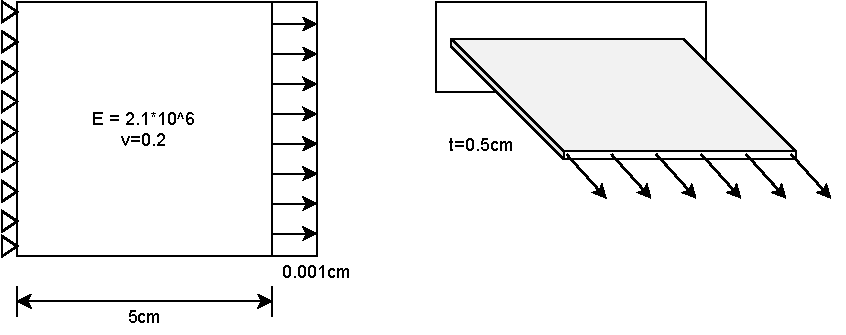
\includegraphics[width=\textwidth]{figuras/placa.pdf}
			\caption{Modelo de placa a tensión, tomado de \textcite{Pisano2009}}
			\label{fig:placa_tension}
		\end{figure}

		Se tienen las siguientes características:
		\begin{enumerate}
			\item[] $a = 5\ cm$
			\item[] $t = 0.5\ cm$
			\item[] $u_0 = 0.001\ cm$
			\item[] $E = 2.1*10^6\ daN/cm^2$
			\item[] $\nu = 0.2$
		\end{enumerate}

		Bajo las siguientes condiciones de borde:
		\begin{enumerate}
			\item[] $U = 0,V=0$ en $x=0$
			\item[] $U = u_0$ en $x=a$
		\end{enumerate}

		Usando el programa, este problema puede modelarse así:

		\begin{figure}
			\centering
			\sffamily
			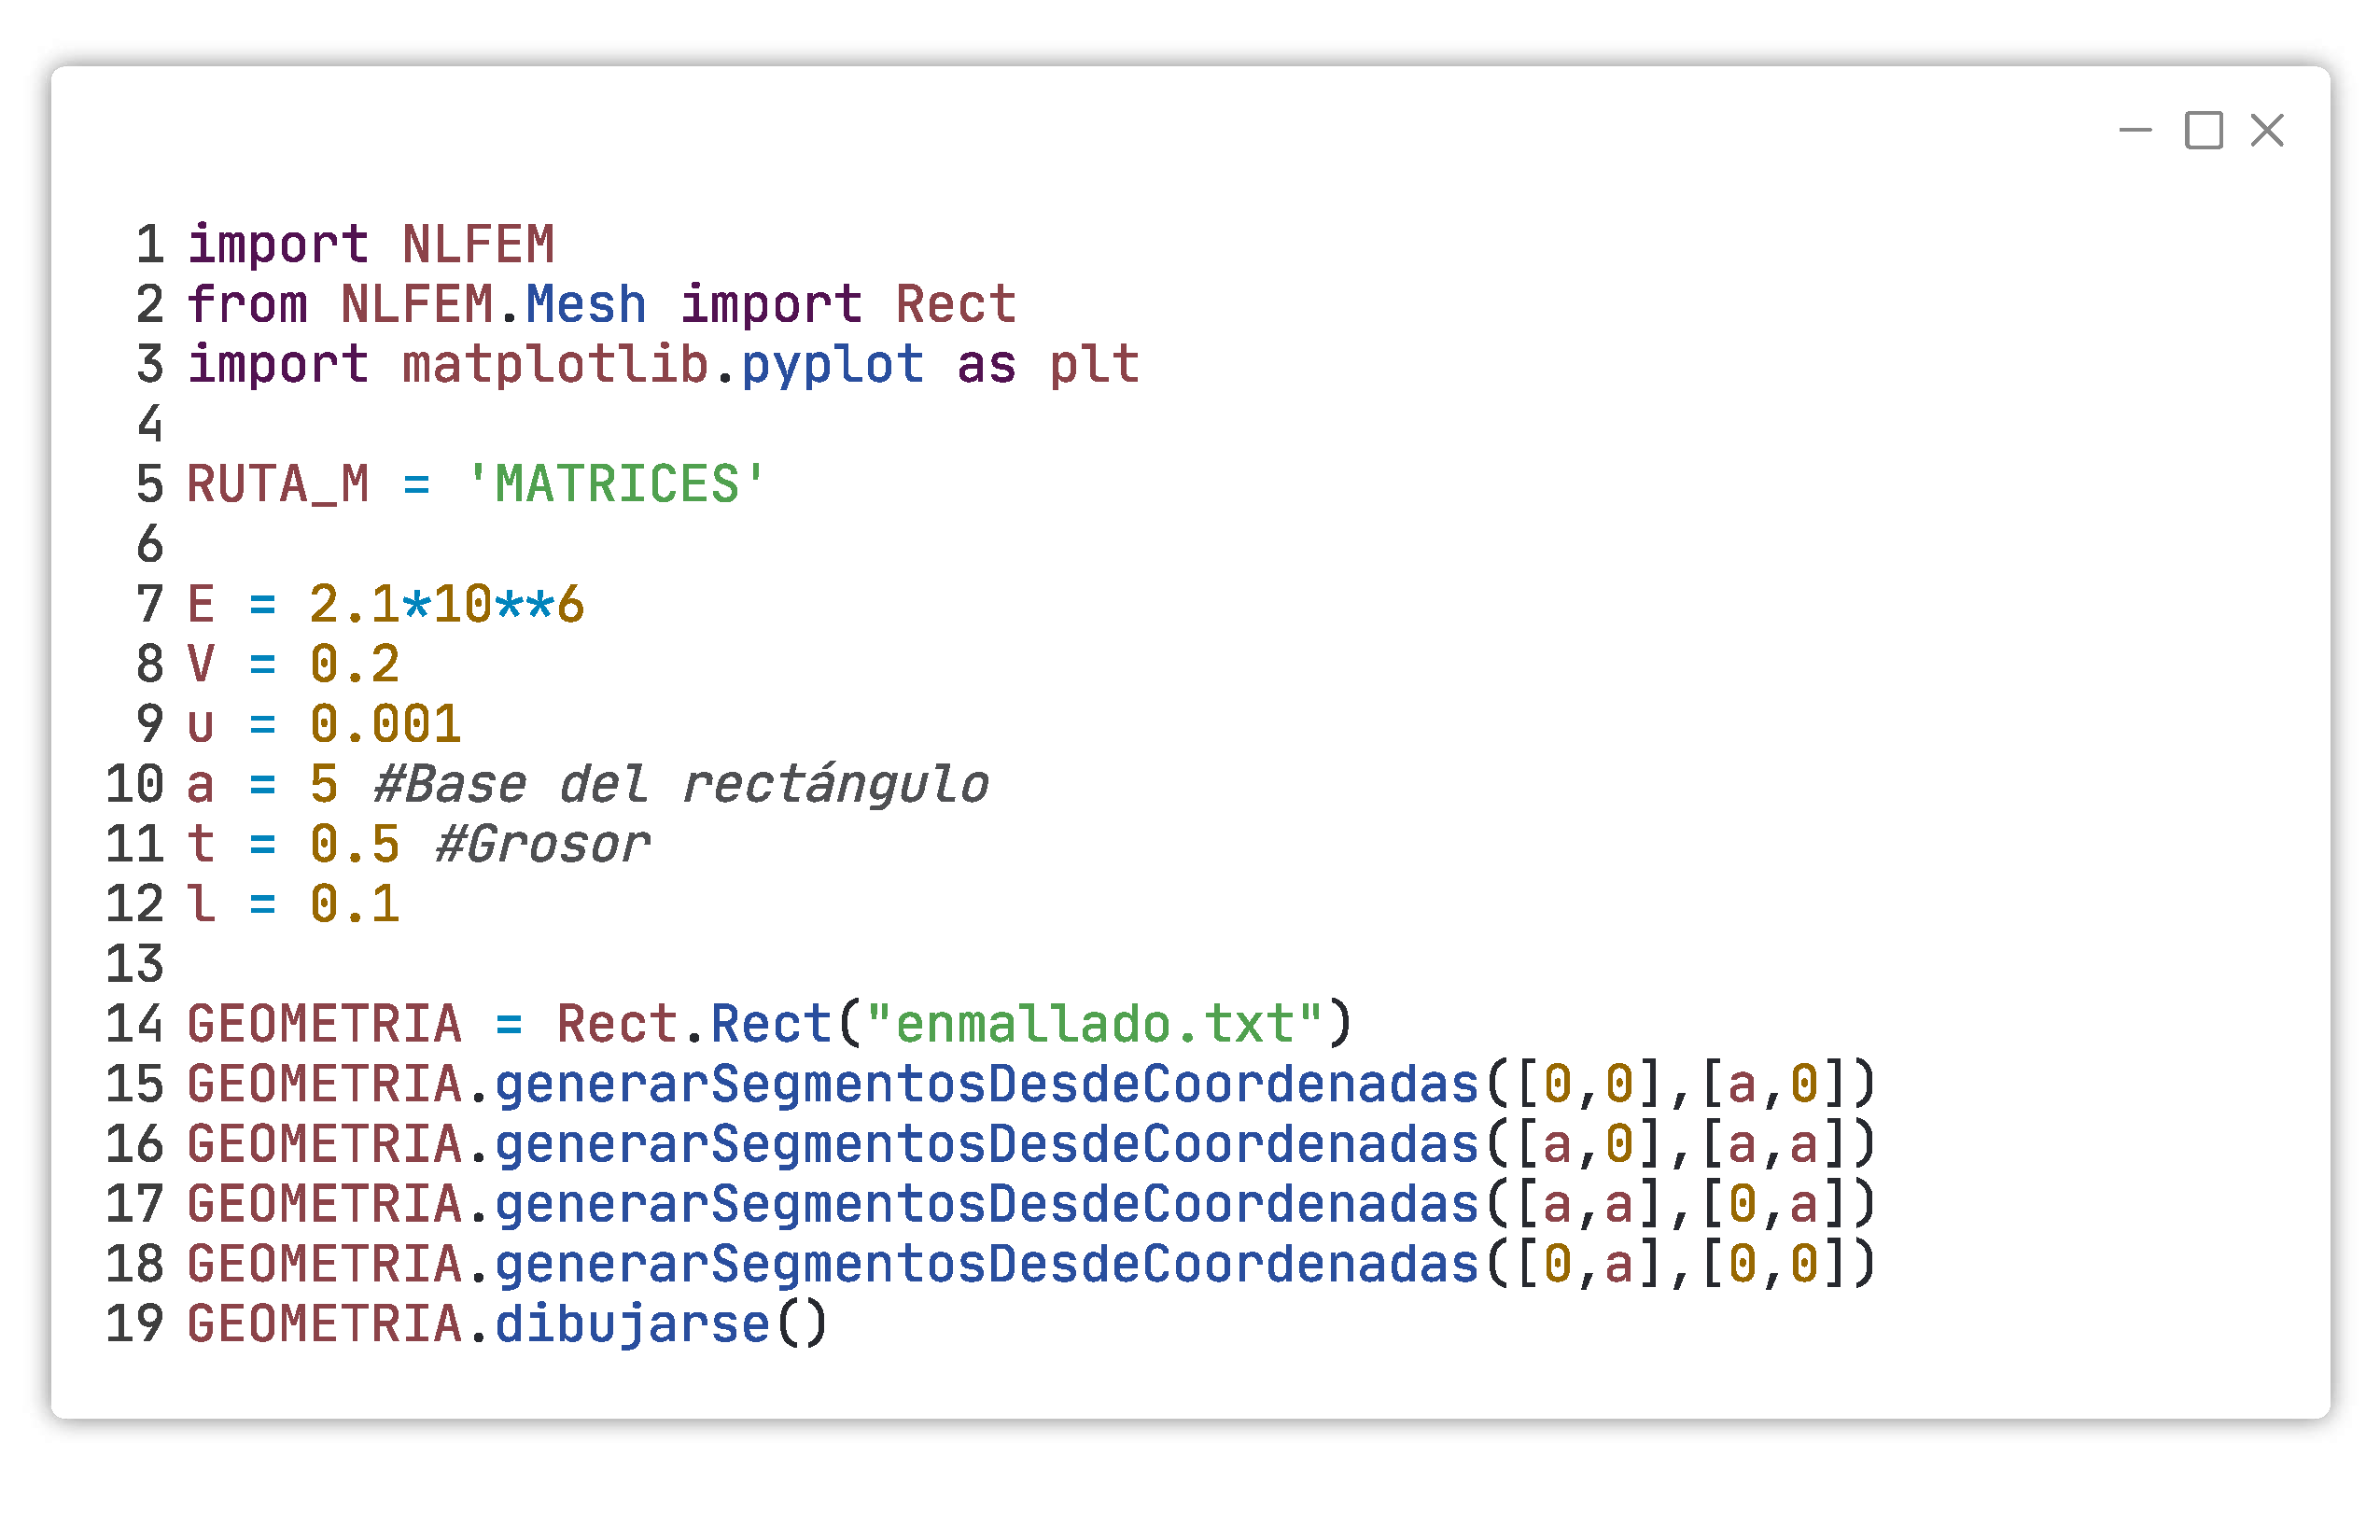
\includegraphics[width=0.9\textwidth]{figuras/placa_c1.pdf}
			\caption{Importar librerías y enmallado}
			\label{fig:imports_placa}
		\end{figure}
		Se importa la librería NLFEM que contiene el programa de NL-FEM completo. Posteriormente, Se definen las variables iniciales del problema, por ejemplo, el módulo de Young, grosor, etc. Se carga la geometría del dominio mediante el archivo \textit{enmallado.txt}, el cual sigue los lineamientos propuestos en la tabla \ref{tab:estructura_enmallado}. Por último, se definen los segmentos que serán de gran ayuda para imponer condiciones de borde. Cada segmento va de un punto inicial a un punto final. El programa encontrará el nodo del enmallado mas cercano a las coordenadas pasadas por parámetro. Finalmente, en la línea 19 se grafíca el enmallado final (la manera en como el programa esta entendiendo el enmallado)

		Para este caso, se trabaja con un enmallado de 100 elementos. El resultado obtenido se aprecia en la figura \ref{fig:enmallado1010placa}

		\begin{figure}
			\centering
			\sffamily
			\scalebox{0.3}{\inputpgf{figuras}{enmallado1010placa.pgf}}
			\caption{Enmallado de 100 elementos para dominio cuadrado.}
			\label{fig:enmallado1010placa}
		\end{figure}

		\begin{figure}
			\centering
			\sffamily
			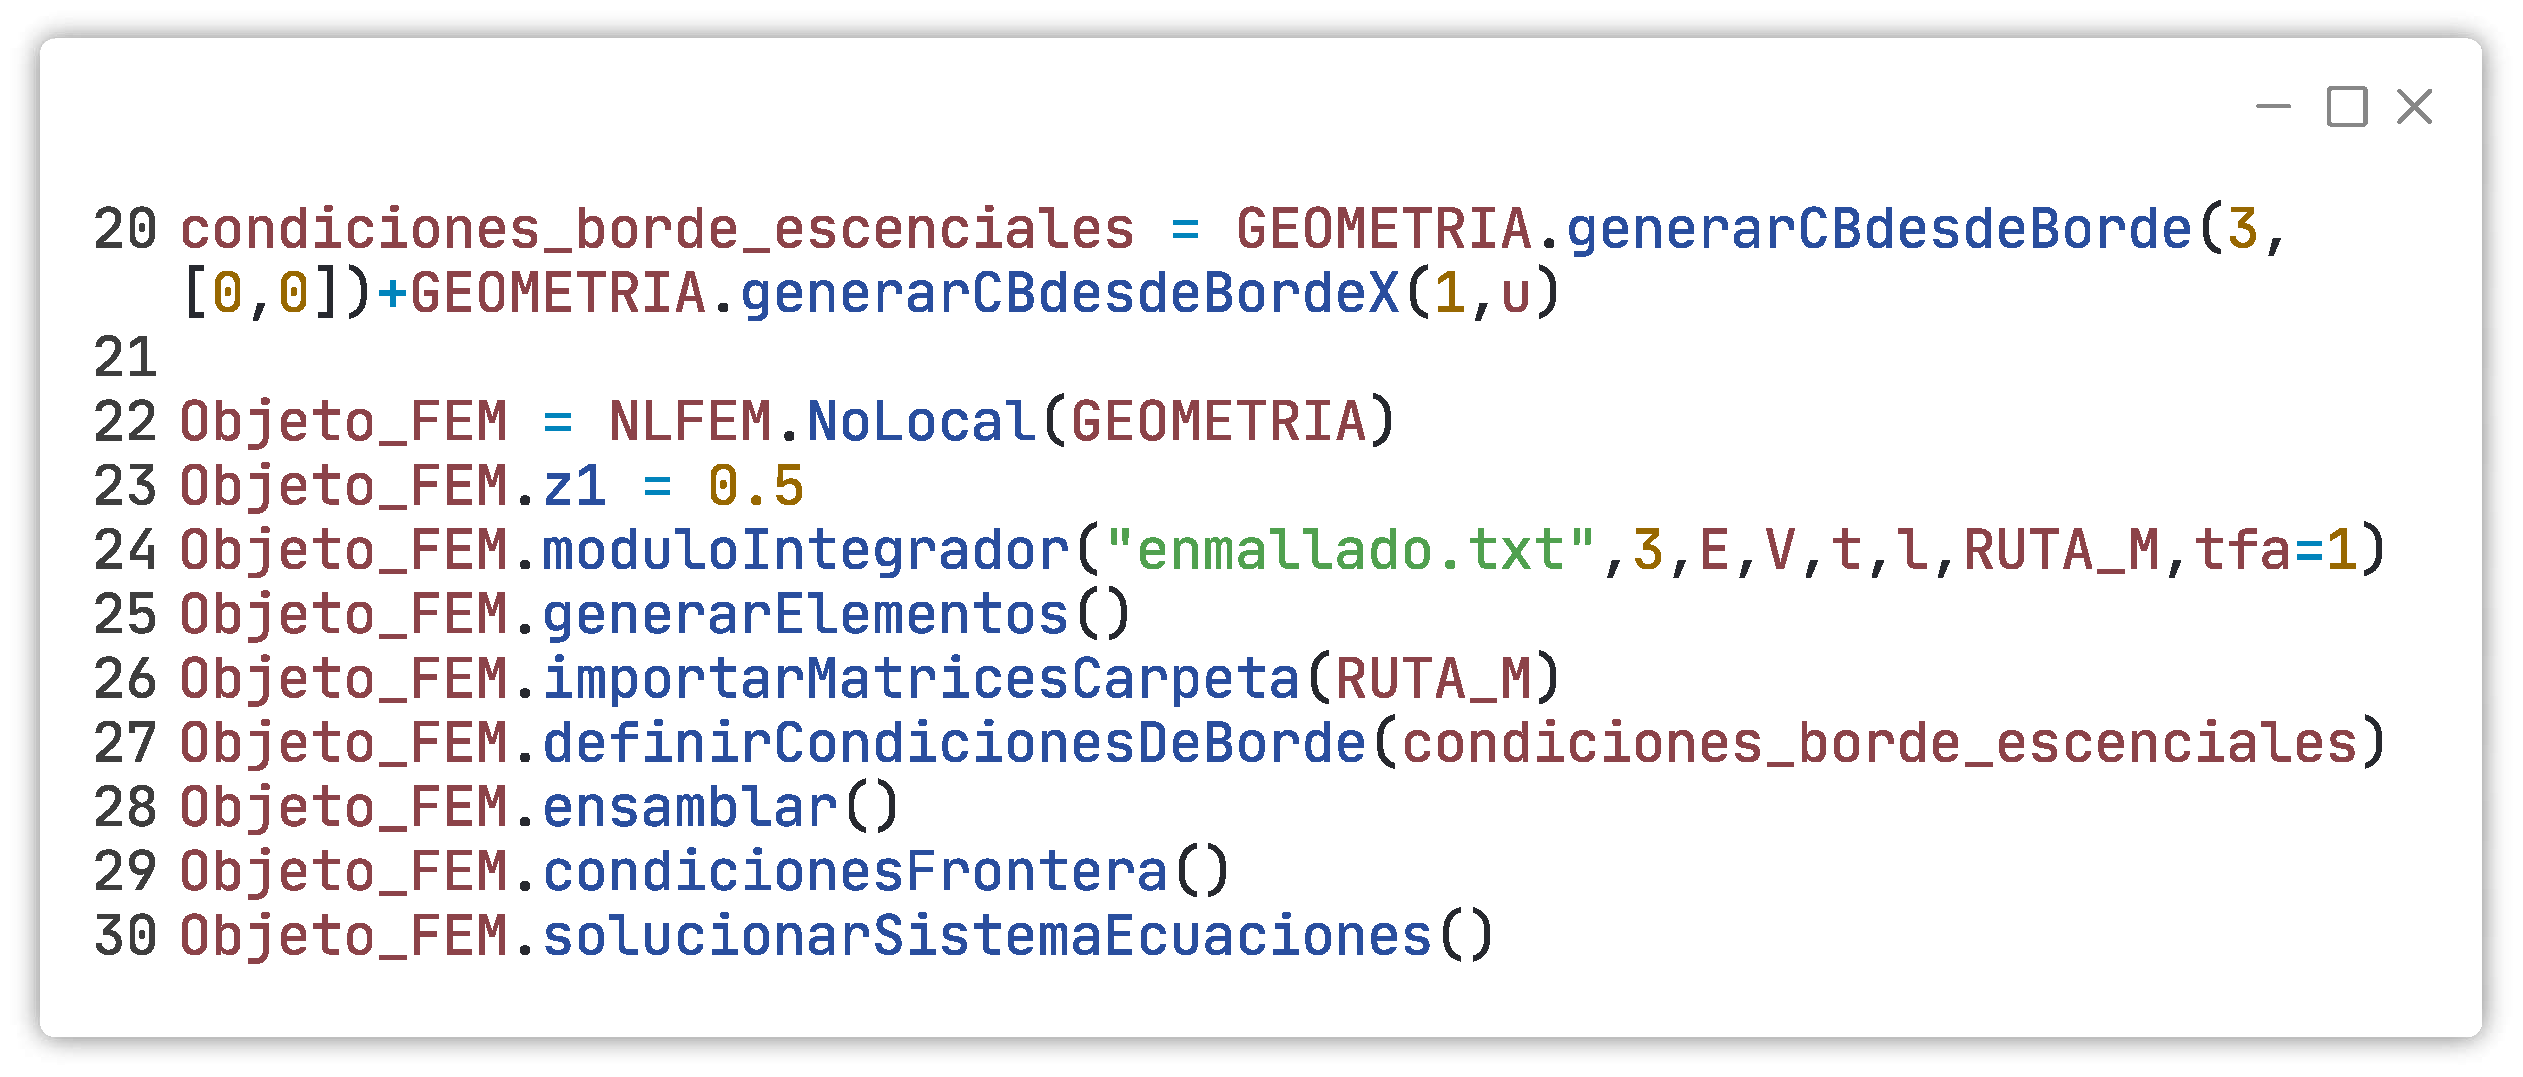
\includegraphics[width=0.9\textwidth]{figuras/placa_c2.pdf}
			\caption{Condiciones de borde integración y solución}
			\label{fig:integracion_ysolucion}
		\end{figure}
		En la línea 20 se nota el proceso de concatenado de las condiciones de borde, las cuales se generan mediante las funciones de la clase \textit{Geometria}. Para este caso, se definen condiciones de borde en los segmentos 3 y 0. Los segmentos pueden observarse en la figura \ref{fig:enmallado1010placa} con color azul. Los bordes se enumeran en el orden en que fueron agregados, lo cual se definió en las líneas 15-18 de la figura \ref{fig:imports_placa}.
		
		Se crea un objeto de la clase \textit{NLFEM} que guarda toda la información necesaria para realizar el proceso. Esta clase toma por parámetro la geometría. En la línea 23 se define el valor para $\zeta_1$ que el programa usará para el ensamblaje de matrices.

		En la línea 24 se llama al módulo integrador. En la carpeta de la variable \textit{RUTA\_M} se generarán los archivos de la integración que siguen el formato propuesto en la figura \ref{fig:archivos_matrices}. Los parámetros del módulo integrador son los definidos previamente. Esta función se encarga de correr el archivo \textit{index.exe} que contiene el codigo de C++ del módulo integrador. Cabe resaltar que este comportamiento solo será válido para Windows. Para otros sistemas operativos se deberá cambiar el archivo index.exe por el archivo compilado desde el código fuente desde C++.

		En las líneas siguientes se ejecutan cada uno de los pasos para NLFEM mencionados anteriormente. Esto resuelve el problema de NL-FEM en el dominio.

		\begin{figure}
			\centering
			\sffamily
			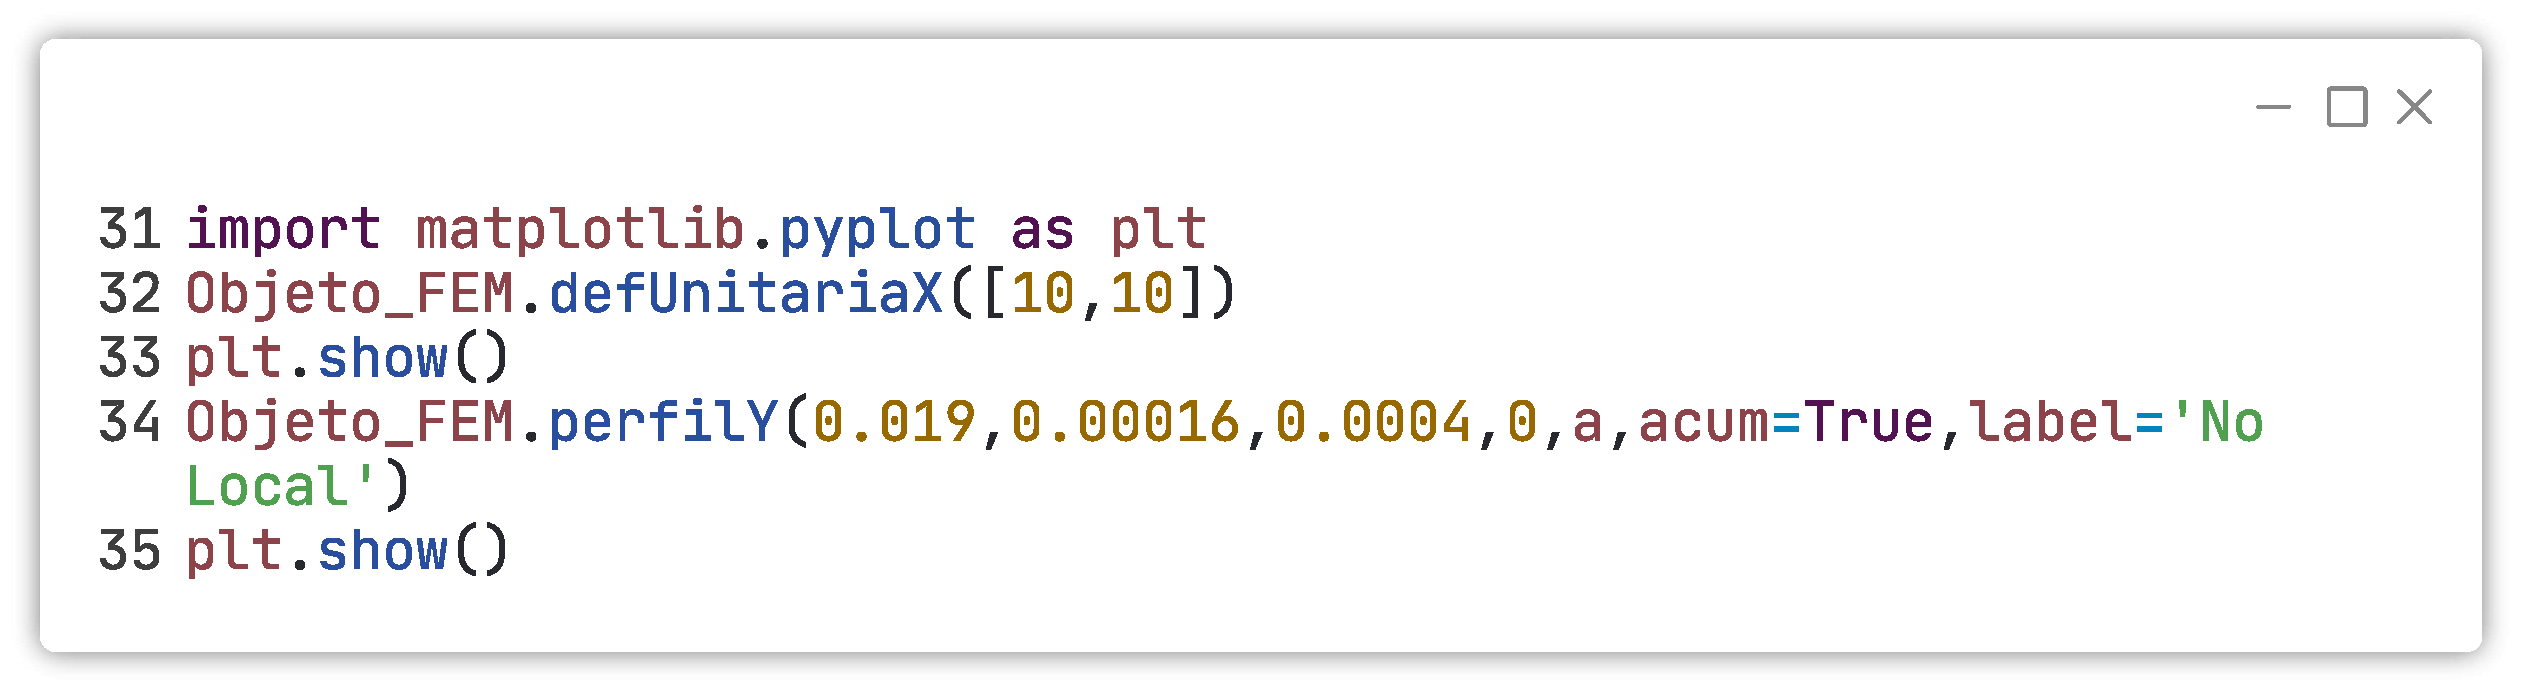
\includegraphics[width=0.9\textwidth]{figuras/placa_c3.pdf}
			\caption{Post proceso}
			\label{fig:postproceso}
		\end{figure}
		El programa permite realizar gráficas de resultados, en la figura \ref{fig:postproceso} se muestran algunos de estas funciones. Las gráficas de resultados se muestran en la figura \ref{fig:resultados_1010}.

		\begin{figure}
		    \centering
		    \sffamily
		    \begin{subfigure}{0.45\textwidth}
		    \centering
			    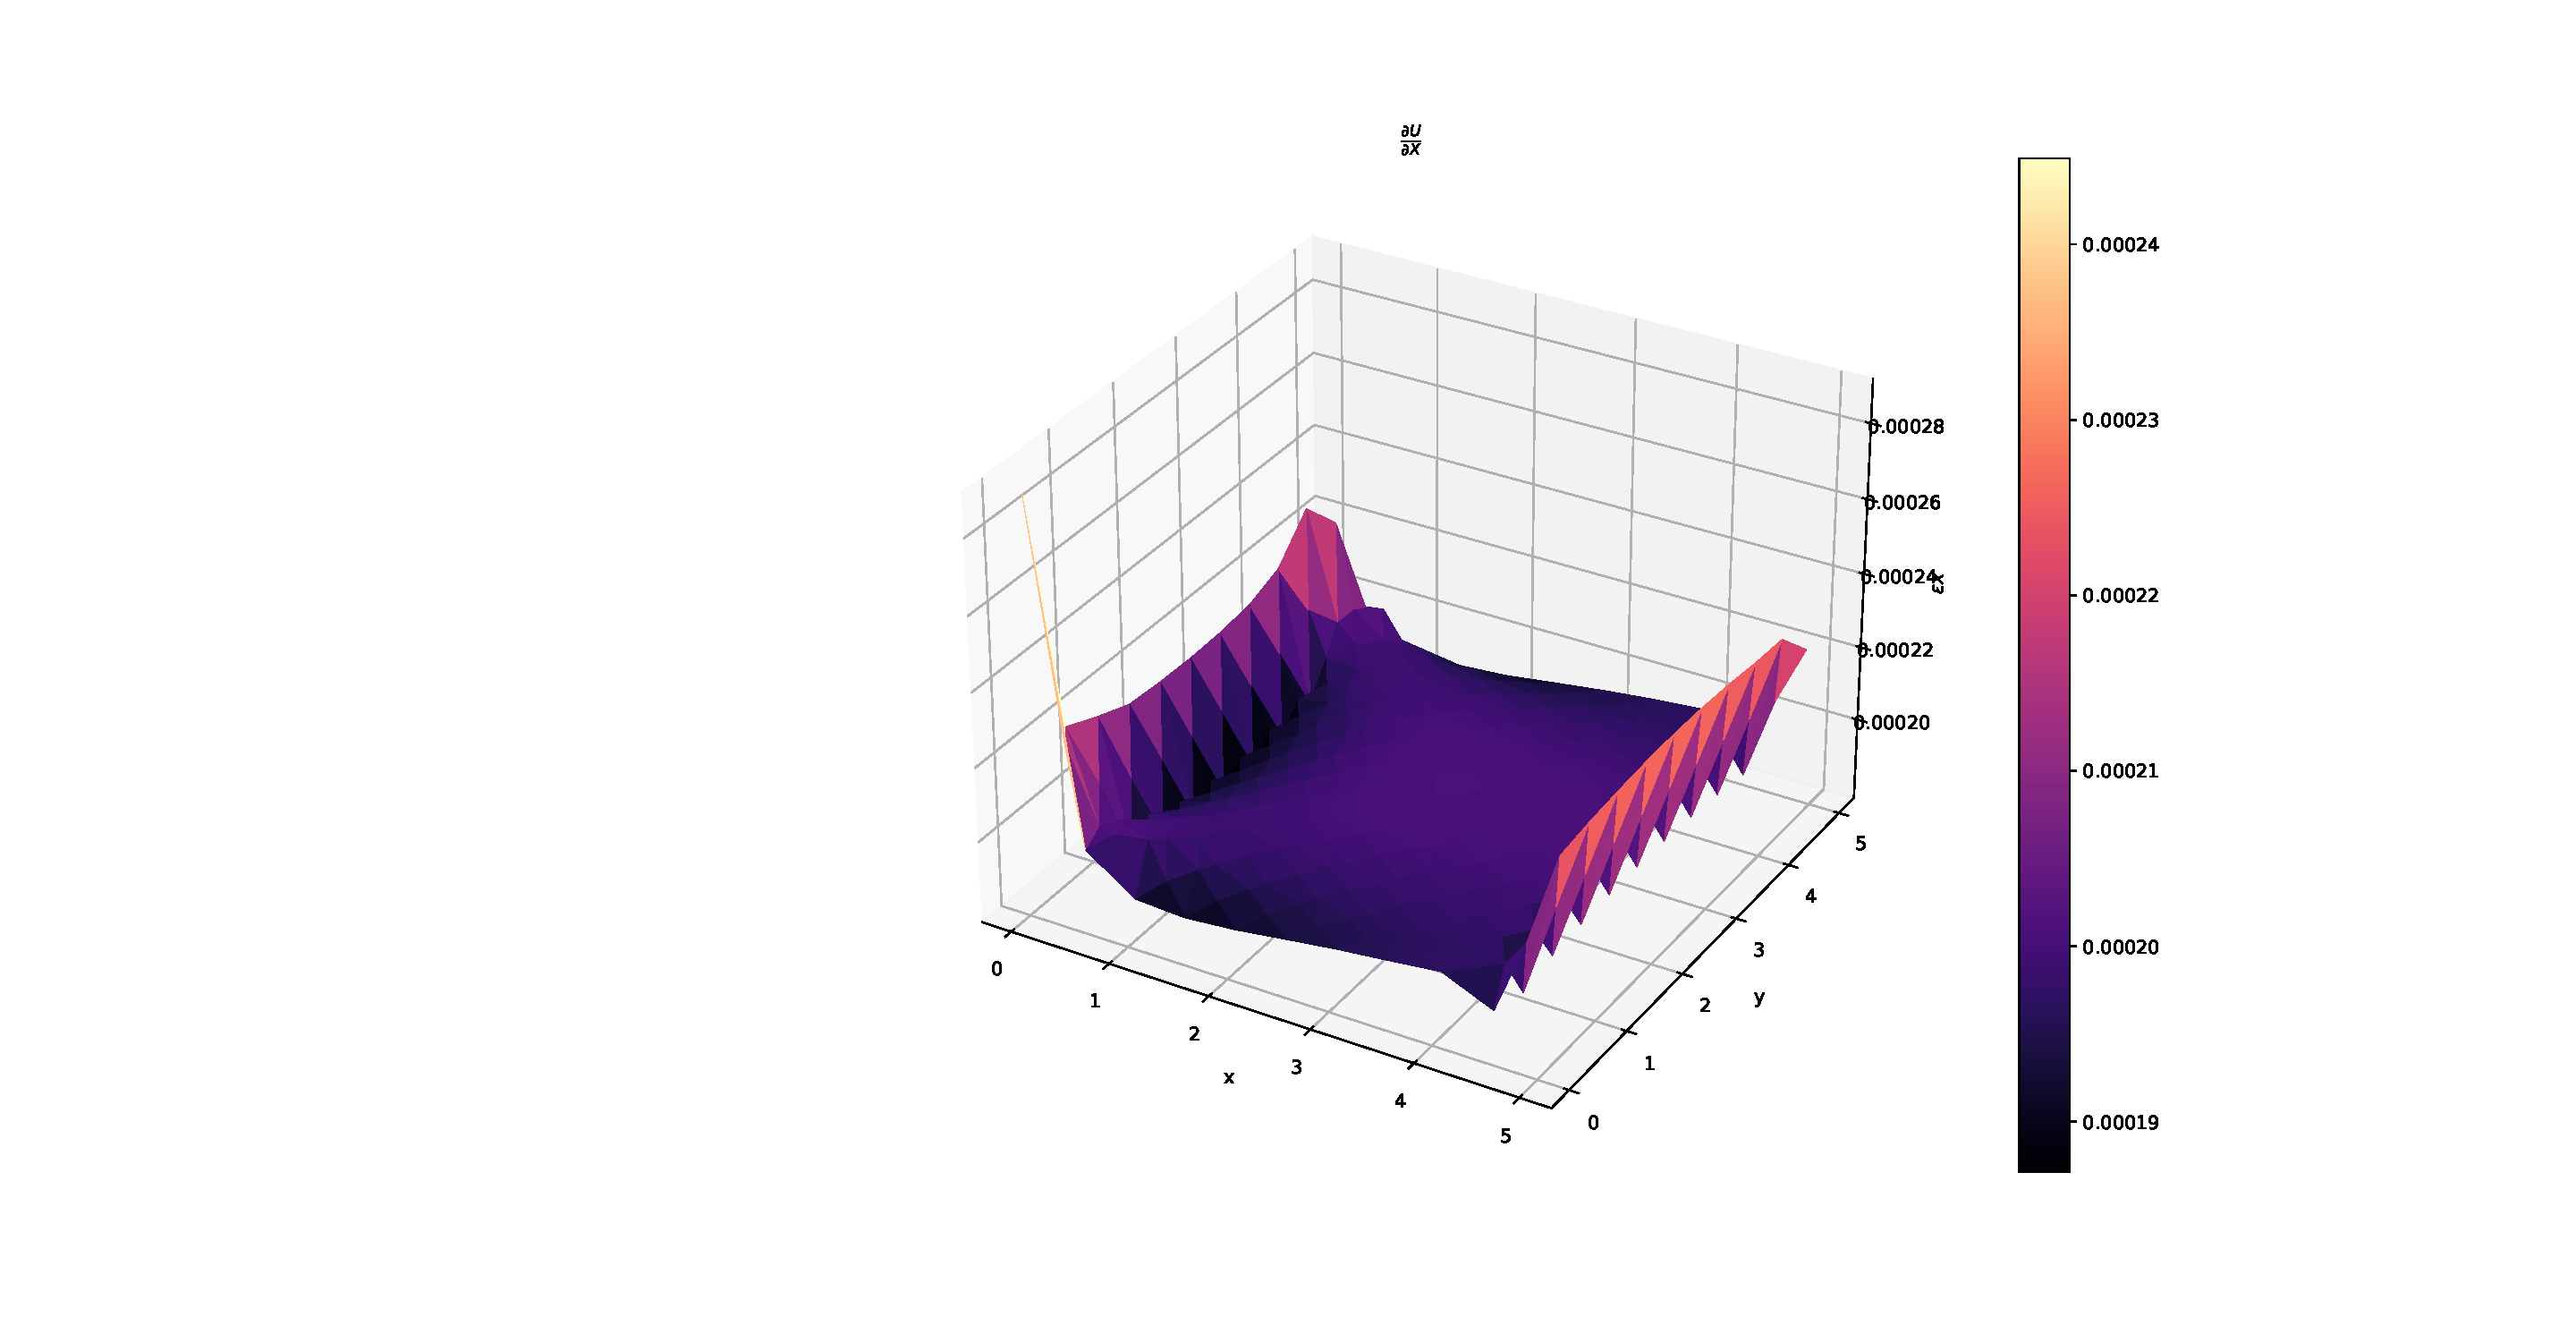
\includegraphics[width=\textwidth]{figuras/enmallado1010placa_defx.pdf}
		        \caption{Superficie de deformaciones ($\varepsilon_x$)}
		        \label{fig:resultados_1010.1}
		    \end{subfigure}
		    \begin{subfigure}{0.45\textwidth}
		    \centering
		    	\scalebox{0.3}{\inputpgf{figuras}{enmallado1010placa_defy.pgf}}
		        \caption{Perfil de deformaciones en $y=0.019$}
		        \label{fig:resultados_1010.2}
		    \end{subfigure}
		    \caption{Resultados gráficos para un enmallado de 100 elementos}
		    \label{fig:resultados_1010}
		\end{figure}

		\item \textbf{Barra a tensión:}

		La barra a tensión se puede modelar como se muestra en la figura \ref{fig:barra_tension}

		\begin{figure}
			\centering
			\sffamily
			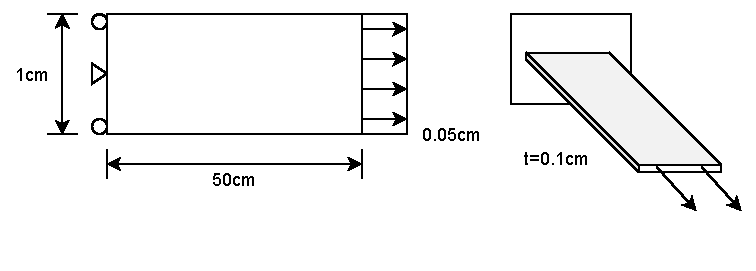
\includegraphics[width=0.6\textwidth]{figuras/barra.pdf}
			\caption{Modelo de barra unidimensional tomado de \textcite{Pisano2009}}
			\label{fig:barra_tension}
		\end{figure}

		Se tienen las siguientes características:
		\begin{enumerate}
			\item[] $L = 50\ cm$
			\item[] $h = 1\ cm$
			\item[] $t = 0.1\ cm$
			\item[] $u_0 = 0.05\ cm$
			\item[] $E = 2.1*10^6\ daN/cm^2$
			\item[] $\nu =0.20$
		\end{enumerate}

		Bajo las siguientes condiciones de borde:
		\begin{enumerate}
			\item[] $U = 0$ en $x=0$
			\item[] $V = 0$ en el punto $x=0,y=h/2$
			\item[] $U = u_0$ en $x=L$
		\end{enumerate}

		Este problema puede ser modelado de la misma manera que el problema anterior, el cambio mas relevante son las condiciones de borde (asumiendo los cambios obvios en propiedades del material y enmallado). Para ello basca con concatenar una condicion de borde puntual con el comando \textit{generarCBYdesdeCoordenada(x,y,valor)} que asignará la condición al nodo mas cercano a la coordenada que se da por parámetro.

	\end{enumerate}
	\subsection{Validación}
	\label{sub:validacion}

	Para realizar la validación de resultados obtenidos, se compararon los perfiles resultantes de correr el programa con los obtenidos por \textcite{Pisano2009}. En la figura \ref{fig:perfiles_validacion} se muestran 4 perfiles obtenidos con el caso de estudio 1 usando una malla de 900 elementos, $\zeta_1=0.5$, $l=0.1$. Para comprobar la validez se realizo una superposición de imágenes entre los perfiles obtenidos y los perfiles propuestos por \textcite{Pisano2009}. Estas gráficas se encuentran en el anexo \ref{fig:anexos.validacion}

	\begin{figure}
	    \centering
	    \sffamily
	    \begin{subfigure}{0.48\textwidth}
	    \centering
	        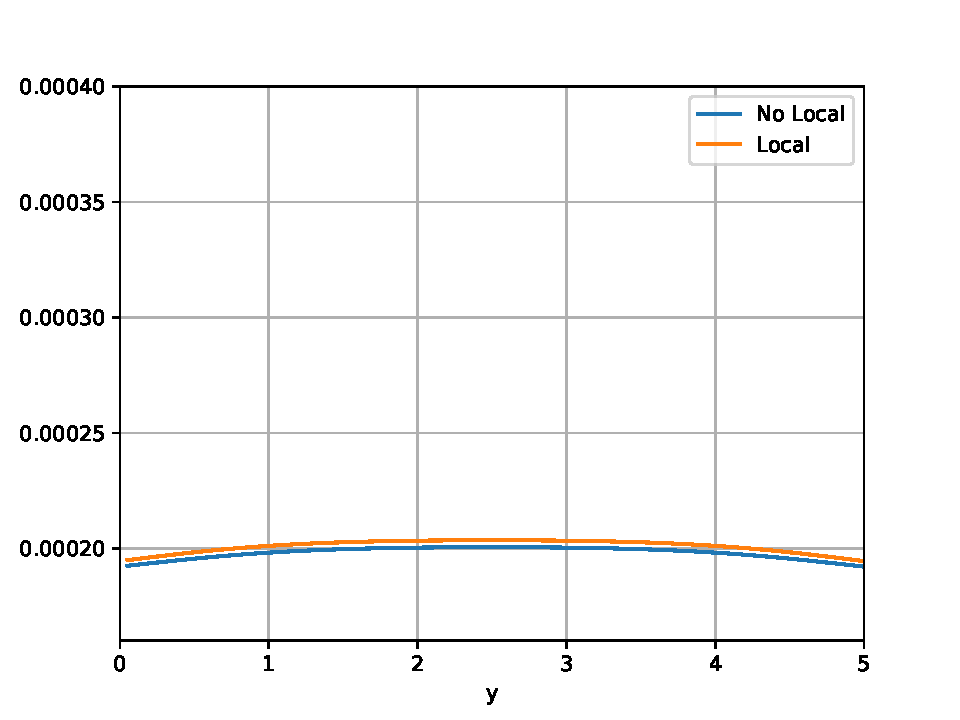
\includegraphics[width=\textwidth]{figuras/PerfilX2519.pdf}
	        \caption{Perfil en $x=2.519$}
	        \label{fig:perfiles_validacion.x2519}
	    \end{subfigure}
	    \begin{subfigure}{0.48\textwidth}
	    \centering
	        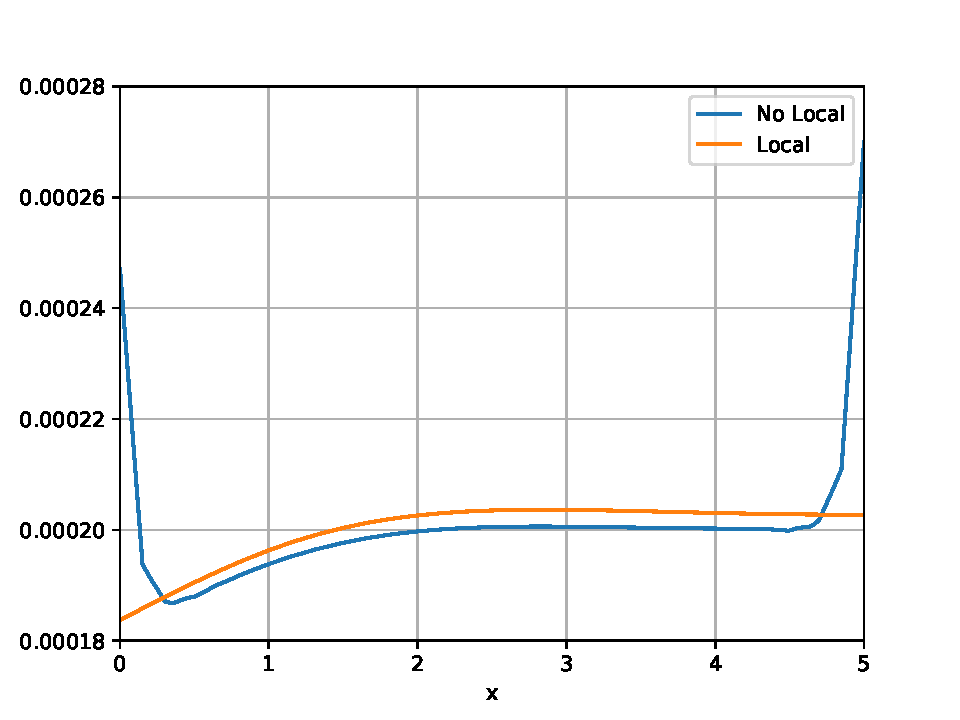
\includegraphics[width=\textwidth]{figuras/PerfilY2519.pdf}
	        \caption{Perfil en $y=2.519$}
	        \label{fig:perfiles_validacion.y2519}
	    \end{subfigure}
	    \quad
	    \begin{subfigure}{0.48\textwidth}
	    \centering
	        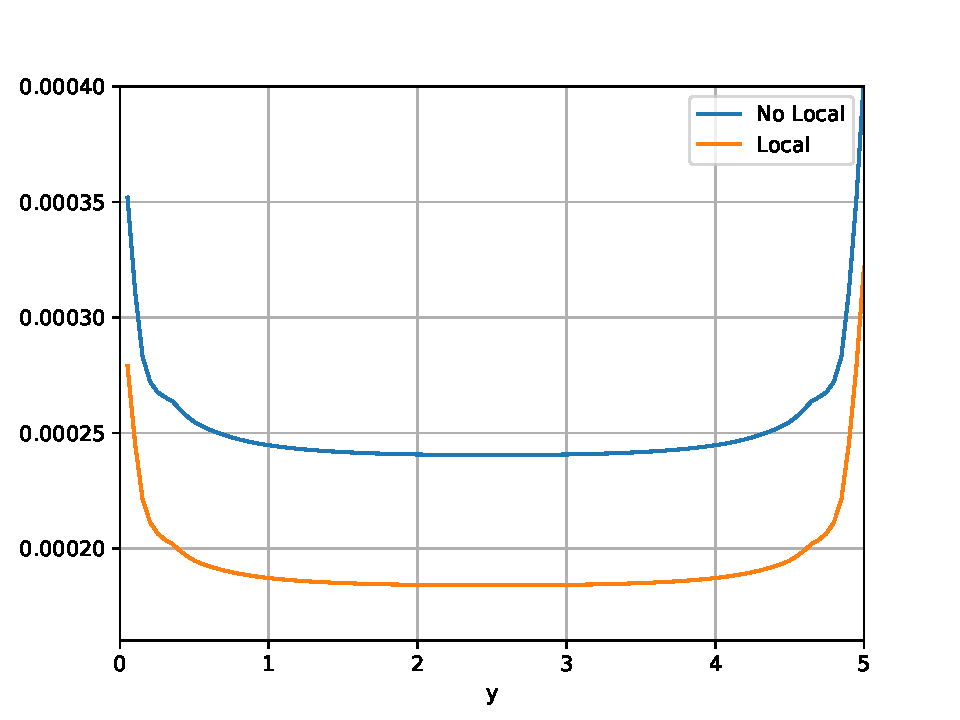
\includegraphics[width=\textwidth]{figuras/PerfilX0019.pdf}
	        \caption{Perfil en $x=0.019$}
	        \label{fig:perfiles_validacion.x0019}
	    \end{subfigure}
	    \begin{subfigure}{0.48\textwidth}
	    \centering
	        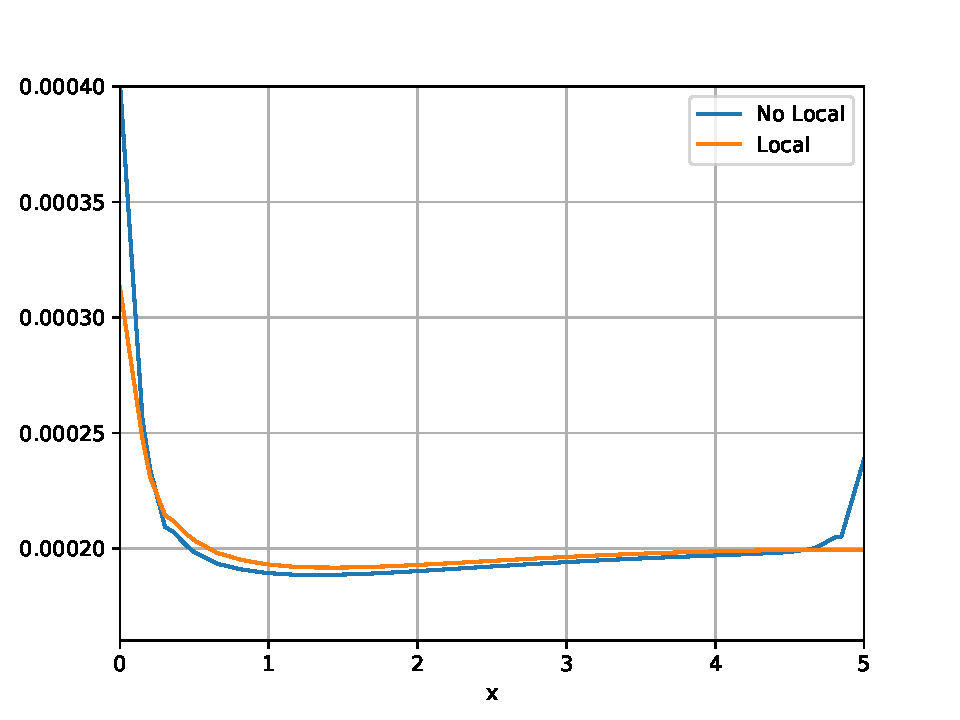
\includegraphics[width=\textwidth]{figuras/PerfilY0019.pdf}
	        \caption{Perfil en $y=0.019$}
	        \label{fig:perfiles_validacion.y0019}
	    \end{subfigure}
	    \caption{Perfiles de $\varepsilon_x$ en el caso de estudio 1}
	    \label{fig:perfiles_validacion}
	\end{figure}

	\subsection{Variación de Parámetros}
	\label{sub:variacion}
		Para generar los resultados se itera condiferentes parámetros, el objetivo de cambiar los parámetros es ver la influencia que tienen en la solución.
		\subsubsection{Variaciones Planteadas}
			\begin{enumerate}
				\item Variación en funciones de atenuación

				El componente principal a evaluar serán las funciones de atenuación. Por tal razon, para cada función de atenuación se extraerán los resultados de forma gráfica. Se usarán las cuatro funciones de atenuación definidas en el capítulo \ref{sc:teoria}
				\item Variación en factor de rigidez ($\zeta_1$)

				El factor de rigidez controla la proporción que tienen los efectos no locales. Dado que se puede expresar como porcentaje, se debe variar de 0 a 1.
				\item Variación en longitud interna ($l$)

				Dado que la longitud interna controla directamente la cantidad de elementos no locales, se estudiarán dos fenómenos. Cuando la cantidad de elementos no locales requeridas por el parámetro $l$ es suficiente en el dominio y cuando la cantidad de elementos no locales requeridas por el parámetro $l$ no es suficiente en el dominio. Por lo tanto, el parametro $l$ varía de 0 a la lonigitud mas pequeña del dominio sobre 12. En el caso del caso de estudio 1 se usara un $l_{max}=\frac{1}{12}$ y en el caso de estudio 2 $l_{max}=\frac{1}{12}$

				En el caso de estudio 1, $l_{max}$ garantiza que para el elemento mas interior hay suficientes elementos adyacentes en un radio $Lr$ lo que garantiza que aunquesea para ese elemento se tenga en cuenta todo el dominio. Los elementos que se encuentren fuera de este radio (las esquinas) no serán relevantes por estar demasiado lejos del elemento de interés \parencite{Polizzotto2001}. 
			\end{enumerate}
	La metodología completa se resume en el diagrama de flujo presentado en la figura \ref{fig:flowchart}

	\begin{figure}
		\centering
		\sffamily
		\includegraphics{figuras/FlujoMetodología.pdf}
		\caption{Diagrama de flujo del proceso iterativo}
		\label{fig:flowchart}
	\end{figure}